%
% Niniejszy plik stanowi przykład formatowania pracy magisterskiej na
% Wydziale MIM UW.  Szkielet użytych poleceń można wykorzystywać do
% woli, np. formatujac wlasna prace.
%
% Zawartosc merytoryczna stanowi oryginalnosiagniecie
% naukowosciowe Marcina Wolinskiego.  Wszelkie prawa zastrzeżone.
%
% Copyright (c) 2001 by Marcin Woliński <M.Wolinski@gust.org.pl>
% Poprawki spowodowane zmianami przepisów - Marcin Szczuka, 1.10.2004
% Poprawki spowodowane zmianami przepisow i ujednolicenie
% - Seweryn Karłowicz, 05.05.2006
% Dodanie wielu autorów i tłumaczenia na angielski - Kuba Pochrybniak, 29.11.2016

% dodaj opcję [licencjacka] dla pracy licencjackiej
% dodaj opcję [en] dla wersji angielskiej (mogą być obie: [licencjacka,en])
\documentclass[licencjacka]{pracamgr}

\usepackage{hyperref}
\usepackage{graphicx}
\usepackage{listings}
\usepackage{xcolor}
\usepackage{textcomp}


\lstset{
  aboveskip=3mm,
  belowskip=3mm,
  showstringspaces=false,
  columns=flexible,
  basicstyle={\small\ttfamily},
  numberstyle=\tiny\color{gray},
  keywordstyle=\color{blue},
  commentstyle=\color{dkgreen},
  stringstyle=\color{mauve},
  breaklines=true,
  breakatwhitespace=true,
  tabsize=4,
  escapeinside=``,
  frame=tb
}

% Dane magistrantów:
\autori{Michał Borkowski}{370727}
\autorii{Jakub Bujak}{370737}
\autoriii{Marian Dziubiak}{370784}
\autoriv{Marek Puzyna}{371359}

\title{Kompilacja NianioLanga do efektywnych konstrukcji języka C}


%\tytulang{An implementation of a difference blabalizer based on the theory of $\sigma$ -- $\rho$ phetors}

%kierunek:
% - matematyka, informacyka, ...
% - Mathematics, Computer Science, ...
\kierunek{informatyka}

% informatyka - nie okreslamy zakresu (opcja zakomentowana)
% matematyka - zakres moze pozostac nieokreslony,
% a jesli ma byc okreslony dla pracy mgr,
% to przyjmuje jedna z wartosci:
% {metod matematycznych w finansach}
% {metod matematycznych w ubezpieczeniach}
% {matematyki stosowanej}
% {nauczania matematyki}
% Dla pracy licencjackiej mamy natomiast
% mozliwosc wpisania takiej wartosci zakresu:
% {Jednoczesnych Studiow Ekonomiczno--Matematycznych}

% \zakres{Tu wpisac, jesli trzeba, jedna z opcji podanych wyzej}

% Praca wykonana pod kierunkiem:
% (podać tytuł/stopień imię i nazwisko opiekuna
% Instytut
% ew. Wydział ew. Uczelnia (jeżeli nie MIM UW))
\opiekun{mgr. Radosława Bartosiaka\\
  Instytut Informatyki\\
  }

% miesiąc i~rok:
\date{Maj 2018}

%Podać dziedzinę wg klasyfikacji Socrates-Erasmus:
\dziedzina{
%11.0 Matematyka, Informatyka:\\
%11.1 Matematyka\\
%11.2 Statystyka\\
11.3 Informatyka\\
%11.4 Sztuczna inteligencja\\
%11.5 Nauki aktuarialne\\
%11.9 Inne nauki matematyczne i informatyczne
}

%Klasyfikacja tematyczna wedlug AMS (matematyka) lub ACM (informatyka)
\klasyfikacja{D. Software\\
  D.3. Programming languages\\
  D.3.3. Language contructs and features}

% Słowa kluczowe:
\keywords{kompilacja, języki programowania, analiza semantyczna,
  NianioLang, system typów}

% Tu jest dobre miejsce na Twoje własne makra i~środowiska:
\newtheorem{defi}{Definicja}[section]

% koniec definicji

\begin{document}

\maketitle

%tu idzie streszczenie na strone poczatkowa
\begin{abstract}
W pracy opisujemy...
\end{abstract}

\tableofcontents
%\listoffigures
%\listoftables

\chapter*{Wprowadzenie}
  \addcontentsline{toc}{chapter}{Wprowadzenie}
  NianioLang jest językiem programowania ogólnego przeznaczenia. Jego twórcą jest
  założyciel firmy Atinea, na zlecenie której realizowana jest poniższa
  praca -- Andrzej Gąsienica-Samek.
  Istniejący kompilator umożliwia translację NianioLanga do kilku języków,
  między innymi do Javy, JavaScriptu i C.
  Ze względu na chęć uproszczenia kompilacji NianioLanga
  utworzono środowisko uruchomieniowe dostarczające odpowiednie abstrakcje
  i pozwalające na korzystanie w C z dynamicznych struktur odpowiadających typom,
  jakie są dostępne do użycia w NianioLangu. Takie rozwiązanie nie jest
  niestety optymalne, szczególnie w przypadku niskopoziomowego języka jakim
  jest C. W tej pracy opisujemy wprowadzenie nowych typów danych i ich wsparcia
  w kompilatorze, co umożliwi generowanie natywnego kodu w C i znacznie
  zwiększy wydajność kompilowanych aplikacji przy zachowaniu podstawowych założeń języka.
\chapter{Wstęp}
\section{Wprowadzenie do NianioLanga}
NianioLang jest proceduralnym, imperatywnym językiem, którego celem jest
uproszczenie pisania rozproszonych aplikacji stosując wzorzec projektowy
Nianio\cite{wzorzec_nianio}.
Celem twórców języka jest dostarczenie narzędzia umożliwiającego operowanie na niemutowalnych strukturach
o semantyce zbliżonej do języków funkcyjnych, ale prostszego w użyciu.
Konstrukcje takie jak wskaźniki zostały usunięte, a w ich miejsce, w przypadku kompilacji do C,
zaimplementowano system zarządzania obiektami
w pamięci przez zliczanie referencji, aby pozbyć sie jednego z najczęstszych źródeł błędów, występujących przy programowaniu niskopoziomowym.
Takie zabiegi zmniejszają nieco wydajność języka, ale jego twórcy doszli do wniosku, że zysk z wysokopoziomowego podejścia
do pisania aplikacji jest wystarczająco duży, aby tworzenie aplikacji w NianioLangu było opłacalne.

Kompilator NianioLanga jest rozwijany przez firmę Atinea, która używa NianioLanga w swoich projektach (m.in. InstaDB.com).
Kod źródłowy kompilatora jest dostępny na platformie GitHub\cite{github_repo_nianiolang_original} na licencji MIT.

\section{Typy w NianioLangu}
W NianioLangu mamy doczynienia z kilkoma wbudowanymi typami. Wszelkie typy tworzone przez użytkownika, to właściwie aliasy na typy wbudowane,
co pomaga w zarządzaniu abstrakcją w programie. Dostępnych jest pięć wbudowancyh typów: 
\begin{itemize}
  \item \texttt{ptd::sim} -- liczby całkowite, zmiennoprzecinkowe oraz ciągi znaków
  \item \texttt{ptd::rec} -- rekordy, czyli odpowiedniki struktur znanych np. z C
  \item \texttt{ptd::hash} -- słowniki o kluczach będących ciągami znaków i wartościach danego typu
  \item \texttt{ptd::var} -- typ wariantowy, który reprezentuje obiekty, mogące być w dokładnie jednym z określonego zbioru stanów i dodatkowo
  zawierać dane o typie właściwym dla danego stanu
  \item \texttt{ptd::arr} -- tablice danych tego samego typu
\end{itemize}

Typy te mogą być ze sobą łączone w bardziej skompilowane konstrukcje, na przykład \texttt{ptd::arr(ptd::sim())} definiuje
typ tablicy wartości prostych, a \texttt{ptd::rec(\{a => ptd::sim(), b => ptd::sim()\})} definiuje typ rekordu o dwóch polach będących wartościami
prostymi.

Podstawowymi założeniami systemu typów w NianioLangu są: niemutowalność struktur i opcjonalne typowanie.

\begin{itemize}
 \item Niemutowalność struktur w NianioLangu jest pojęciem słabszym, niż w językach funkcyjnych. Oznacza ona,
 że język daje gwarancję, iż między dwoma kolejnymi dostępami do zmiennej jej wartość nie ulegnie zmianie.
 W klasycznych językach imperatywnych, posiadających wskaźniki lub referencje nie jest to prawdą -- jeśli istnieją dwa wskaźniki
 do jednej zmiennej, wartość odczytana z jednego z nich może się zmieniać nawet bez jego jawnej modyfikacji.
 \item Opcjonalne typowanie oznacza gwarancję, że dodanie lub usunięcie typów z programu nie zmieni jego semantyki.
 W skrajnym przypadku można usunąć z programu całą informację o typach i będzie on działał bez zmian
 (oczywiście może to być ze szkodą dla łatwości utrzymania lub wydajności). Jest to podejście przeciwne do stosowanego
 w takich językach jak C++, czy Haskell, których złożone systemy typów mają istotny wpływ na semantykę programu.
\end{itemize}

W wielu językach istnieje znacznie więcej wbudowanych typów, jednak powyższe są wystarczające, aby zbudować skomplikowane aplikacje,
a jednocześnie dość proste, żeby rozpoczęcie programowania w NianioLangu nie było dla programisty wyzwaniem.
W rozdziale \hyperref[sec:compiler]{Kompilator NianioLanga} opisana została implementacja powyższych typów w języku C.

\section{Cele projektu}
Celem projektu była modyfikacja kompilatora NianioLanga, w taki sposób, aby kod wynikowy w C zawierał mniejszą liczbę wywołań funkcji oraz
skomplikowanych
struktur dla prostych typów istniejących już w języku C.
Dzięki temu zmniejszony został czas wykonania aplikacji, pozwalając kompilatorowi GCC na zastosowanie dodatkowych optymalizacji.
W tym celu wprowadzone zostały nowe typy z przestrzeni nazw \texttt{own},
które będą bardziej niskopoziomowymi odpowiednikami typów z przestrzeni nazw \texttt{ptd} (rekordy, tablice i warianty).
Dzięki nałożonym na nie ograniczeniom możliwe jest znaczne zwiększenie wydajności programów pisanych w NianioLangu przy zachowaniu
niezmienionej semantyki języka.
Jednocześnie zmienione zostały pewne podstawowe typy, mianowicie \texttt{ptd::sim} został rozbity na
\texttt{ptd::int} oraz \texttt{ptd::string}, oraz wprowadzony został typ \texttt{ptd::bool}.
Liczby całkowite i wartości boole'owskie mają w języku C natywną reprezentację i używając ich bezpośrednio
uzyskujemy prostszy kod wynikowy w C, który jest łatwiejszy do optymalizacji przez kompilator GCC.

Skutkiem zmian jakie musiały zostać wprowadzone by osiągnąć cel projektu było utracenie możliwości
kompilacji NianioLanga do języków innych niż C do czasu implementacji nowych typów w pozostałych językach.
To zadanie pozostaje jednak poza zakresem niniejszej pracy.

\section{Podstawowe pojęcia}

\chapter{Metodyka pracy}
Prace nad kodem prowadzone były regularnie od połowy października do maja,
z wyłączeniem sesji na przełomie lutego i stycznia. Na rysunku \ref{img:commits_over_time}
przedstawiony został wykres zmian, które wpływały na główną gałąź repozytorium kodu.
Co tydzień zespół prezentował swoje poczynania opiekunowi, co dostarczało stałej motywacji
do implementacji kolejnych elementów projektu.

\begin{figure}[h]
  \centering
  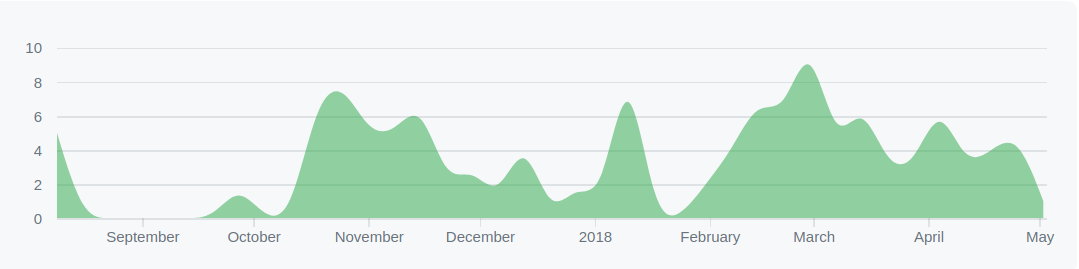
\includegraphics[width=0.9\textwidth]{commits_over_time}
  \caption{Liczba commitów na głównej gałęzi repozytorium w czasie trwania projektu.}
  \label{img:commits_over_time}
\end{figure}

\section{Korzystanie z systemu kontroli wersji}
Podczas pracy zespołowej niezmiernie istotna jest wymiana i zarządzanie fragmentami kodu,
jakie piszą poszczególni członkowie zespołu. Ponieważ każdy w zespole pracował już
wcześniej z systemem kontroli wersji Git, to został on użyty w tym projekcie.
Dodatkowym atutem tego systemu kontroli wersji jest szeroka dostępność darmowych
publicznych repozytoriów kodu online. Kod projektu umieszczony został na portalu
GitHub, który jest największym serwisem pozwalającym na hostowanie kodu online.

Początkowo każdy w zespole miał swoją gałąź w repozytorium, oznaczoną jego imieniem,
na której wprowadzał swoje zmiany. Jednak w trakcie pracy za praktyczniejsze podejście
zostało uznane tworzenie osobnych gałęzi kodu dla każdego zadania.
Umożliwiło to pracę nad kilkoma niezależnymi zadaniami jednocześnie i ułatwiło
przeglądy kodu poprzez tematyczny podział zmian.

GitHub oprócz repozytorium kodu, udostępnia również narzędzia do zarządzania zadaniami
w projekcie, co zostało wykorzystane. Każde duże i średnie zadanie było zapisywane
w systemie zgłoszeń. Po ustaleniu osoby wykonującej zadanie było ono przypisywane
na tę osobę, a po wgraniu zmian na główną gałąz zadanie było zamykane.
Dzięki temu w dowolnej chwili możliwe było określenie nad czym pracuje dany członek
zespołu i jakie otwarte zadania pozostały do przydzielenia.

\section{Zgłaszanie zmian i code review}
Po napisaniu kodu rozwiązującego dane zadanie, zgłaszany był tzw. Pull Request,
czyli żądanie zatwierdzenia zmian. Aby zmiany zostały zatwierdzone i umieszczone
w głównej gałęzi projektu, musiały być zatwierdzone przez conajmniej jednego członka
zespołu, innego niż ten który zgłosił PR. GitHub udostępnia widok naniesionych zmian
wraz z możliwością dodawania komentarzy do konkretnych fragmentów kodu. Możliwy więc
był dialog między recenzentem kodu, a jego twórcą, tak aby ostatecznie zatwierdzone
zmiany spełniały oczekiwania obu stron.

\section{Techniki komunikacji w zespole}
Większość komunikacji w zespole odbywała się online przez portal społecznościowy Facebook.
W początkowej fazie projektu, głównym tematem dyskusji była specyfika języka NianioLang,
z którym większość członków zespołu miała po raz pierwszy styczność.
Na dalszym etapie projektu, na konwersacji grupowej na tym portalu, zespół
ustalał większość detali implementacyjnych przed rozpoczęciem ich wdrażania.
Ten środek komunikacji był najchętniej wykorzystywany ze względu na najkrótszy czas
reakcji członków zespołu.

Drugim kanałem komunikacji były zadania i PRy na GitHubie. Zadania w prosty sposób
opisywały co i kto ma zrobić, a opisy PRów określały co zostało przez daną osobę zrobione.
Ta forma komunikacji w projekcie była najmniej używana.

Ostatnim sposobem komunikacji były cotygodniowe spotkania podczas zajęć z Zespołowego
Projektu Programistycznego, po których zespół spędzał 10-20 minut na dogadywaniu się,
kto wybiera które zadanie, a w przypadku pytań lub problemów, na ich rozwiązaniu.

\chapter{Kompilator NianioLanga}
\label{sec:compiler}
\section{Budowanie drzewa AST}
Pierwszym etapem kompilacji jest parsowanie programu wejściowego do drzewa AST. Takie drzewo jest strukturą przechowującą informacje o składniowej
roli wyrażeń, które przetwarzać można na dalszych etapach kompilacji. Celem jest przetworzenie tekstu programu do postaci przypominającej derywację
gramatyki języka. Chociaż książkowa definicja drzewa AST mówi wyłącznie o składni, kompilator NianioLanga już na tym etapie dokonuje pewnej
podstawowej analizy semantycznej, gdyż wydzielenie tych czynności spowodowałoby dużą duplikację kodu związanego z czynnością obchodzenia drzewa.

\begin{figure}[h]
  \centering
  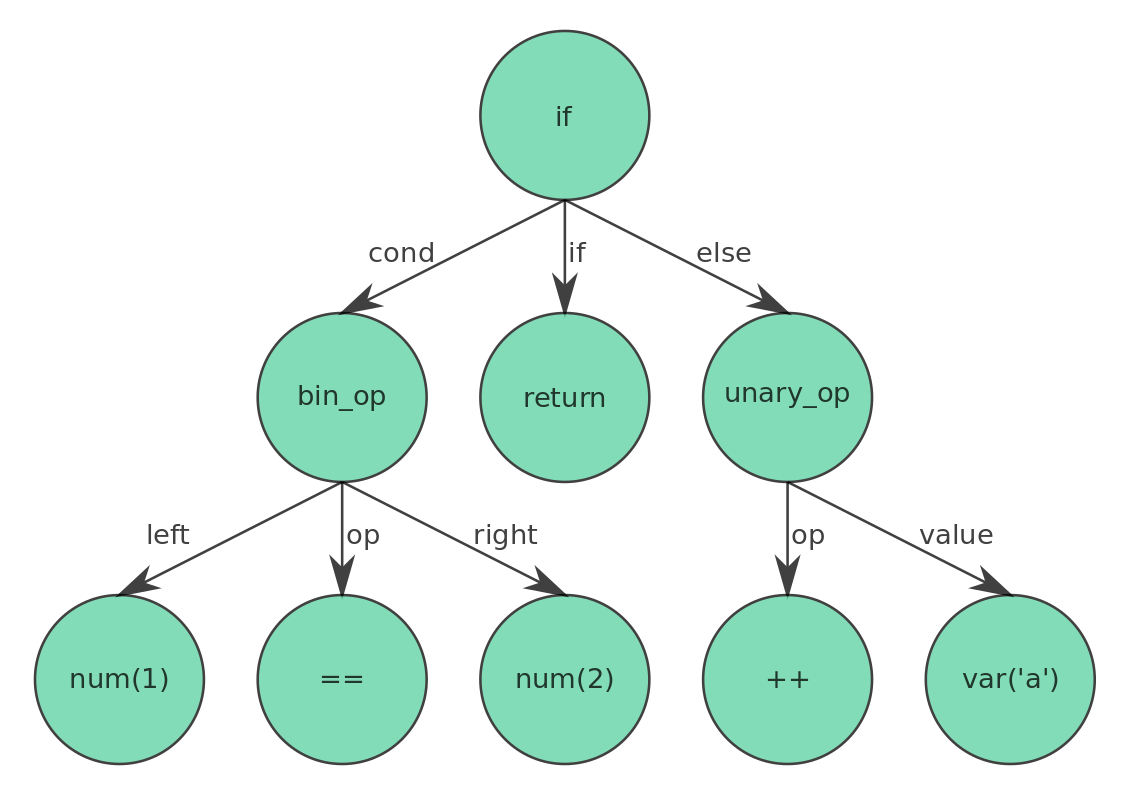
\includegraphics[width=0.6\textwidth]{files/ast.png}
  \caption{Drzewo AST dla programu \texttt{if (1 == 2) \{return;\} else \{a++;\}}}
  \label{img:ast}
\end{figure}

Najpierw parser próbuje przeczytać listę importowanych modułów, gdyż zgodnie ze składnią języka musi ona zostać umieszczona na początku programu. Po
tym etapie następuje parsowanie listy funkcji. Każdy etap parsowania odbywa się poprzez analizę możliwie najdłuższej ilości tekstu, dopisanie błędów,
ustawienie wskaźnika następnej pozycji oraz innych pomocniczych wartości, które są przechowywane w zmiennej reprezentującej stan parsera, a na końcu
zwrócenie sparsowanej wartości. Nie ma znaczenia, co zwróci dana funkcja w razie błędu, gdyż wtedy kompilacja zostanie zatrzymana, a użytkownik
poinformowany o błędzie. W przypadku, gdy nie jest jasne, co należy sparsować (na przykład nie wiadomo, czy oczekujemy kolejnej deklaracji importu
modułu, czy definicji funkcji), próbuje się przeczytać różne wartości, aż któraś zostanie poprawnie sparsowana. Ważne jest, by różne możliwości
przetwarzać od największej do najmniejszej, jeżeli reprezentacja jedna może być początkiem drugiej, np. najpierw parsować należy operatory, a dopiero
potem wyrażenia, chyba że kolejność nie ma znaczenia. Przykładowo w wyrażeniu \emph{1 + 2 - 3} nie ma znaczenia, czy spróbujemy sparsować najpierw
operator dodawania, czy odejmowania, ale operator musi być sparsowany zanim sparsowana zostanie liczba. Innym przykładem jest \texttt{if}, po którym
może nastąpić \texttt{else} i najpierw należy spróbować sparsować blok \texttt{else} zanim przejdzie się do parsowania następnych komend.

Parsowanie funkcji odbywa się poprzez sparsowanie nagłówka, a następnie sparsowanie jej wnętrza jako jednej komendy. Przyjęte jest, że komenda może
być także listą komend, co parsuje się w sposób rekurencyjny. Ułatwia to parsowanie takich komend jak \texttt{for} czy \texttt{if}. Podejście to
umożliwia także tworzenie rekurencyjnych funkcji, z których każda odpowiedzialna jest za jeden element gramatyki języka. Funkcje te sposób działania
opierają na opisanym w poprzednim paragrafie schemacie.

Projekt nie wymagał znaczących zmian na etapie parsowania, dlatego nie zostaną one tutaj omówione. Jedynym wyjątkiem jest dodanie sprawdzania po
sparsowaniu funkcji, czy nie definiuje ona typu, a następnie wpisania tego typu do drzewa. Zostało to jednak wykonane przy użyciu dostępnych już
funkcji. Jest to wykonywane, by na dalszych etapach można było zapytać o dowolny definiowany typ, co ułatwia proces kompilacji. Sytuacja błędna nie
jest jednak obsługiwana, stanie się to dopiero podczas sprawdzania poprawności typów.
\section{Analiza semantyczna}
Drugim etapem kompilacji jest sprawdzenie poprawności typów. Wbrew nazwie etap ten nie ma na celu wyłącznie sprawdzenia, czy program jest poprawny
typowo -- do drzewa programu wpisywane są informacje o uzyskanych typach. Jest to konieczne, by móc dopasować typy NianioLanga do typów języka
wynikowego. Ponadto zachodzi tutaj analiza opisana w rozdziale \hyperref[sec:own_to_im]{Konwersja own $\rightarrow$ im}.

Na tym etapie sprawdza się, czy zaimportowane moduły faktycznie istnieją, czy definicje funkcji nie dublują się, oraz w końcu czy używane typy zgodne
są z oczekiwanymi. Trzeci element rozumiany jest dwojako. Po pierwsze, jeżeli dana zmienna ma zadeklarowany przez użytkownika typ, sprawdza się, czy
używana jest ona wyłącznie przez funkcje, które takiego typu oczekują.  Ze względu na nietrywialny system typów wydzielone są specjalne funkcje
sprawdzające czy i w jakim zakresie dwa typy są zgodne. Przykładowo jeżeli \texttt{im} używany jest w kontekście \texttt{hash}, to zgodnym typem jest
\texttt{hash}. Jeżeli zaś funkcja oczekuje \texttt{int} a podawany jest \texttt{array}, to zgłaszany jest błąd. W tym kontekście o typach myśleć można
jako o zbiorach możliwych wartości, na których wykonywane są operacje, przede wszystkim przecięcia.

Drugie rozumienie, które stosuje type checker, jest podobne do pierwszego, lecz w kontekście wnioskowania typów na podstawie wykonywanych na nich
operacji. Jeżeli dana zmienna inicjalizowana jest jako \texttt{int}, a następnie używana jako \texttt{hash}, to zgłaszany jest błąd. Warto zaznaczyć,
że operacje na typach wywnioskowanych są subtelniejsze, gdyż wiele typów jest konwertowalnych na \texttt{im} oraz w drugą stronę, przez co nie jest
możliwa całkowita, ścisła kontrola typów, ta ma miejsce dopiero w runtime. Ponownie, wydzielone są funkcje operujące na typach w analogii do zbiorów.

Samą budowę type checker ma podobną w pewnym sensie do parsera. W rekurencyjny sposób sprawdzamy, jakie typy mają poszczególne elementy drzewa oraz
czy są one poprawne. Tak jak w parserze zapisane jest, że operator \texttt{+} zawiera słowo kluczowe \texttt{+}, tak odpowiednia funkcja w type
checkerze wie, że argumenty tego operatora muszą mieć typ zwracany \texttt{int}. Ponownie pozwala to na podział funkcji w taki sposób, by każda
dotyczyła jednego, jasno wyszczególnionego elementu.
\section{Architektura nlasma}
nlasm to język stosowany w kompilatorze jako pomost pomiędzy NianioLangiem a językiem wyjściowym, gdyż bezpośrednia kompilacja NianioLanga do C, lub
też innego języka, może okazać się trudna, ponieważ używane struktury językowe znacząco od siebie odbiegają. Umożliwia to w łatwy sposób tworzenie
modułów kompilujących NianioLanga do różnych języków. Taka technika jest szeroko stosowana w świecie kompilatorów, jednym z najszerzej znanych
przykładów jest LLVM. Obecność autorskiego nlasma podyktowana jest przede wszystkim potrzebą języka pośredniego, który z jednej strony będzie możliwie
najprostszy, z drugiej w pewnym sensie zachowa strukturę programu wyjściowego.

Funkcje w nlasmie nie operują na zmiennych, lecz na rejestrach. Każdy rejestr ma swój unikalny w obrębie funkcji numer oraz typ. Także argumenty
funkcji są rejestrami. Wprowadzenie typów do nlasma było jednym z elementów projektu, gdyż o ile poprzednio wszystkie zmienne konwertowane były do
typu \texttt{im}, o tyle teraz przechować należy strukturę typów \texttt{own} czy \texttt{int}. Typy w nlasmie mają charakter wyłącznie informacyjny,
to znaczy nie mają żadnego znaczenia semantycznego.

Najważniejszą cechą nlasma jest nie drzewiasta, lecz liniowa struktura programu. Oznacza to, że argumentami wywołań mogą być wyłącznie rejestry, a nie
zmienne czy inne wywołania. W znacznym stopniu ułatwia to dalszą pracę kompilatora, przede wszystkim z powodu mniejszej liczby niuansów dotyczących na
przykład wartości zwracanych, przez co kod generatora języka docelowego może być znacznie prostszy. Ponadto generowanie kodu może odbywać się w sposób
liniowy, to znaczy każda komenda nlasma może mieć jednoznaczne, proste odzwierciedlenie w języku docelowym. Dzięki temu generator może dokonywać
analizy wyłącznie w zakresie charakterystycznym dla danego języka, na przykład do generatora C zostało wprowadzone sortowanie topologiczne deklaracji
typów.

Inną ważną cechą nlasma, wynikającą częściowo z poprzedniej, jest brak pętli. Translator NianioLanga do nlasm musi rozbić każdą pętlę na etykietę oraz
komendę \texttt{goto}. Takie podejście ułatwia tłumaczenie kodu na język docelowy, gdyż w różnych językach pętle działają w odrobinę inny sposób, zaś
\texttt{goto} tworzy nieskomplikowany, wspólny interfejs.

Ponadto nlasm zawiera polecenia służące do zarządzania pamięcią. Zakłada się, że język docelowy będzie korzystał ze zliczania referencji w celu
zwalniania pamięci. Aby nie pisać tej samej funkcjonalności oddzielnie dla wielu generatorów, nlasm zawiera polecenia mówiące o tym, że licznik
referencji danego rejestru (o ile jest on wskaźnikiem) należy zmniejszyć lub zwiększyć, co można w prosty sposób przełożyć na wywołania innych
języków. Oczywiście, jeżeli generator wybierze inną metodę zarządzania pamięcią, na przykład generując kod Javy, może te polecenia po prostu
zignorować. W przypadku generowania języka z manualnym zarządzaniem pamięcią, na przykład C, polecenia te są bardzo pomocne.


Przykładowe komendy nlasma:
\begin{itemize}
\item \texttt{if\_goto} -- sprawdza wartość w rejestrze. Jeżeli prawda, wykonuje skok pod etykietę
\item \texttt{clear} -- sygnalizuje, że wartość licznika referencji powinna spaść
\item \texttt{call} -- wywołuje funkcję o danej nazwie z danymi rejestrami jako argumentami, zapisuje wynik w danym rejestrze
\item \texttt{move} -- kopiuje wartość między dwoma rejestrami
\end{itemize}
\section{Translacja drzewa AST do nlasma}
\section{Generowanie kodu C na podstawie nlasma}
Jak zostało to omówione w poprzednim rozdziale, \texttt{nlasm} został zaprojektowany z myślą o ułatwieniu dalszej kompilacji. Wobec tego generowanie
kodu C jest bardzo proste.


Pierwszym etapem jest wygenerowanie kodu dla pliku nagłówkowego modułu. Zawiera on między innymi komentarz z informacją o tym, że dany plik został
wygenerowany automatycznie, instrukcje importujące nagłówki C biblioteki standardowej NianioLanga, czy też pewne instrukcje inicjujące, na przykład
ustawiające wartości stałych. Warto wspomnieć, że pliki \texttt{.c} i \texttt{.h} generowane są równolegle, gdyż pozwala to na przetwarzanie zgodnie z
kolejnością semantyczną, to znaczy na przykład generowanie wszelkich informacji o funkcji można oddelegować do raz wywoływanej procedury.


Drugim etapem jest wygenerowanie kodu odpowiedzialnego za obsługę typów, czyli ich deklaracje, definicje oraz potrzebne do obsługi funkcje. Przed
zmianami wprowadzonymi w ramach tego projektu etap ten nie występował, gdyż kod C używał ogólnego typu \texttt{ImmT}, który obsługiwać można
biblioteką standardową NianioLanga. Obecnie, ponieważ dla każdego typu \texttt{own} tworzony jest oddzielny typ na poziomie C, a funkcje go
obsługujące generowane są na poziomie NianioLanga, to podejście zostało zmienione. Ze względu na fakt, że definicje w NianioLangu nie muszą występować
w określonej kolejności, lecz w C już tak, konieczne jest sortowanie topologiczne, z uwzględnieniem możliwości wyodrębnionej deklaracji typu. Jest to
potrzebne do obsługi sytuacji, w której typ \texttt{A} potrzebuje w swojej definicji posługiwać się w pełni typem \texttt{B}, który z kolei posługuje
się wskaźnikiem na typ \texttt{A}.


Trzecim i ostatnim etapem jest wygenerowanie kodu odpowiedzialnego za same funkcje NianioLanga. Komendy nlasm w bardzo prosty sposób tłumaczą się na
język C, wobec czego generator na tym etapie wykonuje niewiele logiki, lecz jedynie pracę związaną z właściwie słownikowym przełożeniem instrukcji
mając jedynie na uwadze pewne szczegóły techniczne. Do tych szczegółów należy, pośród innych pomniejszych zadań, utworzenie wrapperów na funkcje tak,
by można było je wywoływać także mając daną tablicę argumentów, obsługa wskaźników i zarządzanie pamięcią oraz tworzenie komentarzy będących
informacją, której linii oryginalnego programu odpowiada dana seria instrukcji.


Po wykonaniu wszystkich trzech etapów pliki \texttt{.c} i \texttt{.h} danego modułu gotowe są do zapisania na dysku, a kompilator przechodzi do
tłumaczenia kolejnego modułu.
\section{Implementacja typów NianioLanga w C}
\label{sec:c_types_implementation}
Implementacja typów \texttt{ptd} opiera się na generycznym typie \texttt{ImmT}. Typ ten zdefiniowany jest jako \texttt{void*}, a w czasie wykonania
programu wskazuje na konkretne struktury danego obiektu. Pierwsze bajty każdego obiektu zawierają informacje o tym, jaki jest jego typ, oraz jaką
wartość ma licznik referencji. Jest to powszechny schemat symulowania programowania obiektowego w językach, które takowego nie wspierają, a takim
językiem jest C.


Operacje na danych definiowane są przez szereg funkcji dostępnych w bibliotece standardowej NianioLanga, dokompilowywanej do każdego programu, to
znaczy każdy moduł NianioLanga importuje jej nagłówki. Zawierają one podstawową funkcjonalność obsługi arytmetyki, struktur danych, operacji I/O.


Cała obsługa jest dość prosta i ma charakter możliwie najbardziej generyczny, wobec czego jest niezwykle niewydajna, w szczególności w kontekście
operacji na liczbach lub wartościach logicznych. Celem projektu była zmiana tej sytuacji i umożliwienie kompilatorowi C zastosowanie większej liczby
optymalizacji, co opisane jest w kolejnych rozdziałach.

\chapter{Zmiana systemu typów}
\section{Rozdzielenie typu \texttt{ptd::sim}}
\section{Typy \texttt{own}}
  \emph{Jaki jest cel tych typów, ich semantyka, jakie ograniczenia na ich użycie
    nakładamy (w stosunku do typów ptd).}


\chapter{Rozszerzenie nlasma}
\section{Przekazywanie informacji o typach z drzewa AST}
\section{Statyczne sprawdzanie poprawności}

\chapter{Nowe implementacje typów}
\section{Typy proste}
Pierwszą zmianą, jaka została wprowadzona w generatorze kodu, było uproszczenie,
tam gdzie to możliwe, kodu generowanego dla operacji na typach prostych.
Rozdzielenie typu \texttt{ptd::sim} na osobne typy dla liczb naturalnych,
łańcuchów znaków i wartości logicznych umożliwiło bardziej uważny dobór instrukcji języka C,
co przełożyło się na wydajniejszy kod wynikowy.

\subsection{Liczby całkowite}
Wartości typu \texttt{ptd::int}, czyli liczby całkowite, w wyniku wprowadzonych zmian są kompilowane
do zmiennych języka C o typie \texttt{int}. Zapewnia to dobrą wydajność operacji artytmetycznych,
które na obecnych procesorach wykonują się w niewielkiej liczbie cykli. Użycie typu języka C
dedykowanego dla liczb całkowitych umożliwia też kompilatorowi \texttt{gcc} lepszą optymalizację
na dalszym etapie kompilacji (na przykład umożliwia ewaluację stałych w czasie kompilacji).
\subsection{Łańcuchów znaków}
Implementacja łańcuchów znaków nie została zmieniona w stosunku do istniejącej wcześniej.
Decyzja ta była spowodowana efektywnością już istniejącej implementacji -- łańcuchy znaków
są kompilowane to tablic typu \texttt{char[]}, opakowanych w struktury zawierające
rozmiar i pojemność tablicy. Dostęp takich zmiennych odbywa się poprzez specjalne funkcje,
zapewniające utrzymanie poprawnego stanu całej struktury. Jest to minimalny narzut potrzebny żeby
zachować bezpieczeństwo języka i uchronić programistę przed błedami, takimi jak przepełnienie bufora.
Z tego względu została podjęta decyzja o niepowielaniu istniejącej implementacji i wykorzystaniu
tej już istniejącej.
\subsection{Wartości logiczne}
Jak zostało to opisane w rozdziale \hyperref[sec:c_types_implementation]{Implementacja typów NianioLanga w C}, dotychczasowa implementacja wartości logicznych opierała się na dwuwartościowych
języka NianioLang. Z uwagi na to, że warianty są dość wysokopoziomowym mechanizmem, bez
bezpośredniego odzwierciedlenia w języku C, kod wynikowy generowany dla wartości logicznych nie był
efektywny.

W wyniku przeprowadzonych zmian wartości logiczne są kompilowane do zmiennych typu \texttt{bool},
zdefiniowanego w pliku \texttt{stdbool.h} biblioteki standardowej języka C.
Podobnie, jak w przypadku liczb całkowitych zapewnia to dobrą wydajność operacji logicznych
ze względu na bezpośrednie wsparcie procesora i kompilatora \texttt{gcc}.

\subsection{Ograniczenia kompilacji typów prostych}
Z uwagi na leżące u podstaw języka założenie o opcjonalności typów nie było możliwe
zagwarantowanie efektywnej kompilacji typów prostych w każdych warunkach.
Na przykład kod przedstawiony na listingu \ref{lst:immt_variable} zostanie skompilowany do ciągu operacji na mniej efektywnym typie
\texttt{ImmT}. Spowodowane jest to zmianą typu zmiennej \texttt{x} w trakcie działania programu,
przez co nie można jej przypisać żadnego z typów prostych.
\begin{lstlisting}[caption={Zmienna kompilowana do typu \texttt{ImmT}},label={lst:immt_variable}]
var x;
x = 'a';
x = 1;
x++;
\end{lstlisting}

\section{Typy złożone}
Dla każdego typu złożonego z przestrzeni \texttt{ptd} został utworzony odpowiadający mu typ
w przestrzeni \texttt{own}. Dla każdego konkretnego typu, zdefiniowanego przez użytkownika
i korzystającego z typów \texttt{own}, w kodzie wynikowym w C generowane są oddzielne definicje
typu oraz funkcji na nim operujących. Jest to główna różnica w stosunku do typów z przestrzeni
\texttt{ptd}, dla których zdefiniowany był jeden polimorficzny typ \texttt{ImmT}.
Takie podejście umożliwia bardziej efektywną alokację pamięci przez kompilator (ponieważ rozmiar
wielu struktur jest z góry znany) oraz zapewnia statyczną kontrolę typów także przez kompilator
\texttt{gcc}, pozwalając wykrywać wiele błędów w kodzie generowanym przez kompilator
NianioLanga już na etapie kompilacji.
\subsection{Tablice}
Definicje typów \texttt{own::arr} kompilowane są do struktury zawierającej rozmiar tablicy, jej
maksymalną pojemność i wskaźnik na jej pierwszy element. Do programu wynikowego
dodawane są również funkcje,
pozwalające na dodawanie nowego elementu na koniec tablicy, pobieranie wskaźnika do elementu
o danych indeksie oraz na pobieranie rozmiaru tablicy. Operacja dodawania elementu na koniec tablicy
została zaimplmentowana w sposób opisany na przykład w książce
\textit{Wprowadzenie do algorytmów} \cite{cormen}: po przekroczeniu połowy dostępnego miejsca
tablica zostaje powiększona dwukrotnie. Dzięki takiej implmementacji operacja
ta działa w zamortyzowanym czasie stałym.

Dla każdego typu tablicowego zostaje także wygenerowana funkcja zwalniająca pamięć zajmowaną
przez tablicę. Wywołuje ona odpowiednią funkcję zwalniającą pamięć dla każdego elementu,
a następnie zwalnia pamięć, w której znajdowały się elementy tablicy.
\subsection{Rekordy}
\subsection{Typy wariantowe}
\subsection{Hashe}
\section{Konwersja own $\rightarrow$ im}
\label{sec:own_to_im}
Konwersja typów \texttt{own} na typ \texttt{ptd::im}, który jest uniwersalną reprezentacją typów z przestrzeni \texttt{ptd},
jest naturalną potrzebą języka. Obiekty o typie z przestrzeni nazw \texttt{own} są ograniczone w zasięgu,
więc chcąc zwrócić wartość takiego obiektu lub przekazać do funkcji, która przyjmuje argumenty z przestrzeni
nazw \texttt{ptd}, musimy go przekonwertować.

Analiza przypadków użycia konwersji pokazała, że konwersja z typów \texttt{ptd} na typy \texttt{own} nie ma 
szczególnego zastosowania i nie musi być przez język obsługiwana, przede wszystkim dlatego,
że tworzenie typu statycznego z typu dynamicznego w pewnym sensie mija się z celem korzystania z typów statycznych w ogóle,
gdyż narzut wydajnościowy związany z tworzeniem obiektów typu \texttt{ptd::im}, a potem konstruowanie z nich obiektów typu \texttt{own} byłby zbyt duży.
W drugą stronę zaś konwersja pozwala na łączenie nowego kodu ze starym oraz odejście od statycznego typowania w chwili,
gdy chcemy korzystać z funkcji obsługujących wiele typów, na przykład implementując kontenery.

Istnieje wiele sposobów na implementację konwersji. Pierwszy z nich polega na zapisaniu w bibliotece C języka ogólnej funkcji konwertujących obiekty \texttt{own} na obiekty \texttt{ptd::im}.
Podejście to ma jednak wiele wad, przede wszystkim trudność implementacji, dużą podatność na błędy oraz wątpliwą przenośność rozwiązania.
Szczególnie trzeci argument jest ważny, gdyż dalsze kierunki rozwoju języka prawdopodobnie przewidują przywrócenie do kompilatora możliwości kompilowania na inne języki niż C.

Drugi sposób polega na stworzeniu funkcji-wydmuszki przyjmującej w argumencie obiekt \texttt{own}, która w trakcie kompilacji podmieniana jest na właściwy kod dokonujący konstrukcji obiektu \texttt{ptd::im}.
Duże problemy stwarza jednak implementacja dla typów rekurencyjnych (warianty) oraz puchnięcie kodu wynikowego, zawierającego bardzo podobne, potencjalnie bardzo długie sekcje.

Trzeci sposób, który został zrealizowany, jest niejako połączeniem dwóch poprzednich -- dla każdego typu
nazwanego oraz dla każdego typu, który korzysta z funkcji-wydmuszki, generowana jest funkcja,
podpinana w miejsce wydmuszki. Można to w pewnym sensie porównać do generowania szablonów w C++, aczkolwiek ten system jest bardziej wyspecjalizowany.

Pierwszym elementem rozwiązania jest zebranie informacji o tym, jakie funkcje należy wygenerować,
co przeprowadzane jest w dwóch miejscach.
Ze względu na możliwość używania typów z innych modułów, niż w danym momencie wykonywany, każdy moduł udostępniać musi komplet funkcji do rzutowania typów, które definiuje.
Najpierw, po załadowaniu drzewa AST modułu do type checkera, dokonywany jest obchód po funkcjach definiujących typy sprawdzający, czy nie definiują one typów \texttt{own}.
Miejsce to zostało wybrane, gdyż jest to pierwsze miejsce, gdzie pojawia się konkretna wiedza o typach zmiennych.
Następnie, podczas sprawdzania typów funkcji, za każdym razem, gdy napotykana jest funkcja-wydmuszka, zapamiętywany jest typ argumentu, z jakim została ona wywołana.
Typy te są również rekurencyjnie sprawdzane, czy nie zawierają innych typów \texttt{own}, do których także należy stworzyć stosowne funkcje.

Drugim elementem rozwiązania jest generowanie kodu. Tworzona jest zmienna tekstowa, która następnie wypełniana jest instrukcjami tworzącymi obiekt \texttt{ptd::im}.
Ponieważ typy mogą być zagnieżdżone, w razie potrzeb wywołują one inne funkcje konwertujące wewnętrzne obiekty \texttt{own} na \texttt{im}.
Warto podkreślić, że w przypadku typów \texttt{own::rec} oraz \texttt{own::var} funkcje rzutujące nawet podobne typy są istotnie różne.
Rzutując rekordy należy explicite przypisać wszystkie pola, nie jest możliwe zrobienie tego w ogólny sposób pętlą, zaś rzutując warianty
wykonać należy pełną instrukcję \texttt{match}.

Trzecim elementem jest wstrzyknięcie kodu. Sprawdzanie typów rozdzielone jest od wpisywania ich do drzewa AST
i w trakcie tego wpisywania podmieniane są wywołania funkcji-wydmuszki na wywołania
odpowiedniej funkcji o automatycznie generowanej nazwie. Generowana nazwa jest tworzona na postawie nazwy dla typów nazwanych, oraz na podstawie zawartości
dla typów anonimowych -- uzyskujemy w ten sposób deduplikację kodu, generując w kodzie wynikowym C tylko jedną funkcję dla danego typu.

Pozostaje jeszcze problem dodania definicji nowych funkcji do drzewa AST. Wygenerowany kod jest parsowany do samodzielnego modułu,
który przechodzi przez type checker w sposób podobny do normalnego kodu. Po przejściu przez type checker moduły są łączone w jeden. Gdy cały program przejdzie przez type checker
dalsza kompilacja przebiega tak, jak gdyby użytkownik sam utworzył sztucznie wygenerowane funkcje.

Generując funkcje, a z nich drzewo AST, można mieć wątpliwości, czy nie lepiej byłoby od razu tworzyć gotowe do podczepienia poddrzewa, czy nawet kod wynikowy w C,
zamiast marnować czas procesora na przejście przez parser i type checker. 
Zautomatyzowane tworzenie drzewa AST daje gwarancję, że w przypadku dalszej ewolucji kompilatora nie trzeba będzie pamiętać o tym,
aby każda zmiana miała odzwierciedlenie w module generowania kodu. Ze względu na dużą dynamikę rozwoju języka jest to cecha pożądana.
Ponadto zmniejszanie czasu kompilacji programów nie było głównym celem projektu, a analiza przypadków użycia wykazała, że narzut czasowy jest w pełni akceptowalny.

\chapter{Efekty optymalizacji i wnioski}
\section{Porównanie czasu wykonania programów}

\chapter{Wkład poszczególnych członków zespołu}
\emph{Co zrobiliśmy w rozbiciu na osoby}


\appendix

\begin{thebibliography}{99}
\addcontentsline{toc}{chapter}{Bibliografia}

\bibitem{wzorzec_nianio} \href{https://www.mimuw.edu.pl/~chrzaszc/BPJ20067/nianio.pdf}{LK, \textit{Wzorzec ,,Nianio'' przykład} - 2006}.
\bibitem{github_repo_nianiolang_original} \href{https://github.com/nianiolang/nl}{NianioLang Compiler - GitHub}
\bibitem{cormen} Thomas H. Cormen, Charles E. Leiserson, Ron Rivest, Clifford Stein \textit{Wprowadzenie do algorytmów}, Wydawnictwo Naukowe PWN (2013)


\end{thebibliography}

\end{document}


%%% Local Variables:
%%% mode: latex
%%% TeX-master: t
%%% coding: latin-2
%%% End:
